\documentclass[10pt]{article}
\usepackage{icmlko}

\icmlmeta{IP 파운데이션 월드모델}{87}{어제의 0.39는 0.006이었다}{노트 86의 헤드라인을 철회한다 --- 신경망이 작은 도메인을 외운 것을 실력으로 읽었다}

\begin{document}

\twocolumn[
\icmlheader

\begin{abstract}
노트 86이 ``무라벨 전제의 값이 팝업에서 0.39''라고 적었다. 그 수는 인코더가
팝업 라벨 75건을 \emph{전부 보고} 학습한 뒤 최종 능형만 교차검증한 값이었다.
정직하게 다시 쟀다 --- \textbf{인코더 학습에도 폴드를 지켜} 그 폴드의 라벨을
빼고 학습한 뒤 그 폴드를 투영한다. \textbf{팝업이 $+$0.3199에서 $+$0.3260이다.
값은 0.39가 아니라 0.006이다.} 아이돌도 $+$0.7986이 $+$0.3901로 내려온다.
\textbf{노트 86의 헤드라인을 철회한다.} 그리고 왜 그랬는지가 깨끗하다 ---
낙관 편향(낙관 $-$ 정직)이 도메인 크기와 \textbf{$r=-$0.857}로 붙는다. 팝업(75건)
$+$0.384, 아이돌(81건) $+$0.409, 모바일(2,000건) $-$0.000이다. \textbf{노트 86은
가장 작은 두 도메인의 수를 헤드라인으로 삼았고, 거기가 편향이 가장 큰
자리였다.} 남는 것도 있다. 정직한 값의 열 도메인 평균이 $+$0.3772에서
\textbf{$+$0.4144}로 $+$0.0372이고, 이는 현행 인자 공간($+$0.4038)도 넘는다.
그리고 값이 표본 크기와 $r=+$0.480으로 붙는다 --- \textbf{라벨은 표본이 클 때만
값을 한다}(애니 2,073건 $+$0.147, 팝업 75건 $+$0.006). 노트 75 · 86이 다른
길로 낸 결론과 같은 자리다.
\end{abstract}
]

\begin{figure*}[t]
\centering
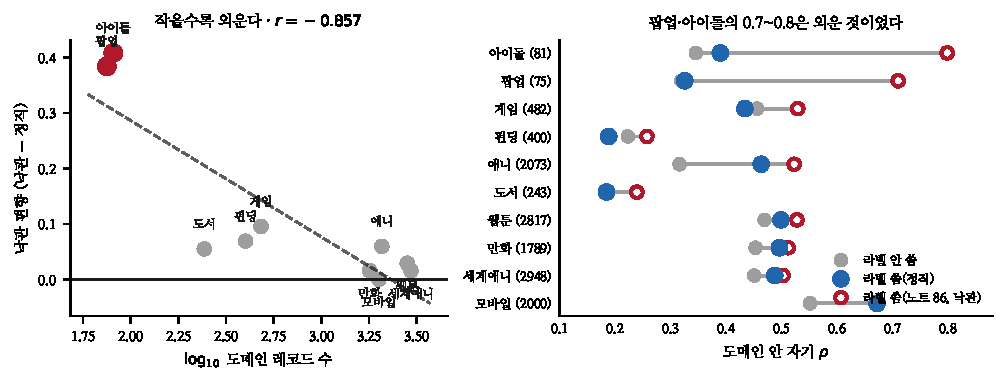
\includegraphics[width=\textwidth]{figs/mem.pdf}
\caption{왼쪽 --- 낙관 편향과 표본 크기. 오른쪽 --- 도메인별 세 값.}
\end{figure*}

\section{정직하게 다시 쟀다}

노트 86의 ``라벨 씀'' 절차는 이랬다 --- 인코더를 \emph{모든} 도메인의 라벨로
학습하고, 그 뒤 잠재$\to$라벨 능형만 5폴드 교차검증했다. \textbf{인코더가
이미 라벨을 봤으므로 잠재 자체에 정답이 새어 있다.}

\begin{quote}\fontsize{9.5}{11.5}\selectfont
고쳤다. 도메인 $d$를 3폴드로 나누고, 폴드마다 \textbf{그 폴드의 라벨을 빼고
인코더를 학습}한 뒤 학습된 인코더로 그 폴드를 투영한다. 능형도 학습 폴드에서만
적합한다. 인코더가 평가 레코드의 라벨을 한 번도 안 본다.
\end{quote}

\begin{table}[t]
\centering\tsize
\caption{도메인 안 자기 $\rho$. 세 절차.}
\begin{tabular}{lrrrr}
\toprule
& $n$ & 라벨 안 씀 & \textbf{정직} & 노트 86 \\
\midrule
\textbf{팝업} & 75 & $+$0.3199 & \textbf{$+$0.3260} & $+$0.7104 \\
\textbf{아이돌} & 81 & $+$0.3461 & \textbf{$+$0.3901} & $+$0.7986 \\
도서 & 243 & $+$0.1840 & $+$0.1851 & $+$0.2399 \\
펀딩 & 400 & $+$0.2235 & $+$0.1890 & $+$0.2578 \\
게임 & 482 & $+$0.4564 & $+$0.4343 & $+$0.5296 \\
만화 & 1789 & $+$0.4535 & $+$0.4964 & $+$0.5124 \\
모바일 & 2000 & $+$0.5518 & $+$0.6725 & $+$0.6724 \\
애니 & 2073 & $+$0.3166 & $+$0.4636 & $+$0.5231 \\
웹툰 & 2817 & $+$0.4697 & $+$0.4993 & $+$0.5282 \\
세계애니 & 2948 & $+$0.4510 & $+$0.4880 & $+$0.5032 \\
\midrule
\textbf{평균} & & $+$0.3772 & \textbf{$+$0.4144} & $+$0.5276 \\
\bottomrule
\end{tabular}
\end{table}

\claimx{노트 86의 ``무라벨 전제의 값이 팝업에서 0.39''를 철회한다. 정직하게
재면 $+$0.3199$\to+$0.3260으로 \textbf{0.006}이다. 아이돌도 0.45가 아니라
0.044다.}{3폴드다. 5폴드나 leave-one-out 이면 조금 다를 수 있는데, 방향이
바뀔 크기는 아니다 --- 팝업 편향이 $+$0.384였다.}

\section{왜 그랬나 --- 작을수록 외운다}

\begin{table}[t]
\centering\tsize
\caption{낙관 편향(노트 86 $-$ 정직).}
\begin{tabular}{lrr}
\toprule
& $n$ & 편향 \\
\midrule
\textbf{아이돌} & 81 & \textbf{$+$0.409} \\
\textbf{팝업} & 75 & \textbf{$+$0.384} \\
게임 & 482 & $+$0.095 \\
펀딩 & 400 & $+$0.069 \\
애니 & 2073 & $+$0.060 \\
도서 & 243 & $+$0.055 \\
웹툰 & 2817 & $+$0.029 \\
만화 & 1789 & $+$0.016 \\
세계애니 & 2948 & $+$0.015 \\
모바일 & 2000 & $-$0.000 \\
\bottomrule
\end{tabular}
\end{table}

$\log_{10} n$ 과 편향의 상관이 \textbf{$-$0.857}이다. 열 점에서 거의 직선이다.

\claimx{신경망의 도메인 안 성적은 그 도메인이 작을수록 낙관적이다 ---
$\log_{10}n$ 과 편향이 $r=-$0.857이다. 팝업(75건) · 아이돌(81건)에서 $+$0.4쯤,
2,000건대에서 0이다.}{편향을 ``외움''으로 불렀지만 인코더는 공유다 --- 작은
도메인의 레코드가 전체의 0.6\%인데도 편향이 크다. 도메인별 머리가 외우는
것으로 보이는데 갈라 확인하지 않았다.}

\begin{quote}\fontsize{9.5}{11.5}\selectfont
\textbf{노트 86은 가장 작은 두 도메인의 수를 헤드라인으로 삼았다.} 그리고 거기가
편향이 가장 큰 자리였다. 이 프로젝트가 여러 번 되풀이한 실수의 신경망 판이다
--- 노트 4의 선택 편향, 노트 67의 작은 표본 배선, 노트 82의 분모 효과.
\end{quote}

\section{남는 것}

철회하고도 남는 것이 둘이다.

\begin{table}[t]
\centering\tsize
\caption{정직한 값과 표본 크기.}
\begin{tabular}{lrr}
\toprule
& $n$ & 값 \\
\midrule
\textbf{애니} & 2073 & \textbf{$+$0.147} \\
\textbf{모바일} & 2000 & \textbf{$+$0.121} \\
만화 & 1789 & $+$0.043 \\
아이돌 & 81 & $+$0.044 \\
세계애니 & 2948 & $+$0.037 \\
웹툰 & 2817 & $+$0.030 \\
도서 & 243 & $+$0.001 \\
\textbf{팝업} & 75 & \textbf{$+$0.006} \\
게임 & 482 & $-$0.022 \\
펀딩 & 400 & $-$0.035 \\
\bottomrule
\end{tabular}
\end{table}

\textbf{첫째, 평균은 여전히 오른다} --- $+$0.3772에서 $+$0.4144다. 그리고 그
값이 현행 인자 공간($+$0.4038)도 넘는다. 대상 라벨을 쓸 수 있으면 인코더가
파이프라인보다 낫다.

\textbf{둘째, 값이 표본 크기와 붙는다} --- $\log_{10}n$ 과 $r=+$0.480이다.
2,000건대 도메인이 $+$0.12$\sim+$0.15를 얻고 75건 팝업은 $+$0.006이다.

\claimx{라벨은 표본이 클 때만 값을 한다. 팝업 75건에서 라벨의 값은 0.006으로
사실상 0이고, 2,000건대에서 $+$0.12$\sim+$0.15다.}{도메인마다 라벨 종류와
축 구성이 달라 표본 크기만의 효과가 아닐 수 있다. 게임 · 펀딩은 표본이
400$\sim$500인데 값이 음수다.}

노트 75가 ``팝업 510건이면 설계 결정을 판정할 수 있다''고 했고 노트 86이
``전제를 풀려면 수백 건''이라 했다. 이 노트가 세 번째 길로 같은 자리에 닿는다
--- \textbf{팝업 표본이 커지기 전에는 팝업 라벨이 아무것도 안 산다.}

\section{한계}

\begin{itemize}[leftmargin=1.1em,itemsep=0.15em]
\item 3폴드다. 폴드가 적으면 학습 표본이 3분의 2로 줄어 정직값이 아래로
      편향된다 --- 진값은 $+$0.4144보다 조금 높을 것이다.
\item 편향을 ``도메인별 머리가 외운다''로 추정했으나 확인 안 했다. 머리를
      빼고 공유 인코더만으로 재면 갈릴 것이다.
\item 게임 · 펀딩에서 값이 음수인 이유를 모른다.
\item 정직한 인코더($+$0.4144)가 현행($+$0.4038)을 넘지만 그것은 \textbf{대상
      라벨을 쓰는} 모형이라 전이 모형과 비교 대상이 아니다.
\item 노트 86의 제품 실험(과거 16건)은 애초에 정직한 절차였고 그 결론
      ($+$0.5192$\to+$0.3866, 내려간다)은 유효하다.
\end{itemize}

\section{다음}

\begin{enumerate}[leftmargin=1.3em,itemsep=0.15em]
\item \textbf{작은 도메인의 신경망 수치를 전부 재검한다} --- 노트 60--62 · 85 ·
      86에서 인코더 관련 수치 중 팝업 · 아이돌이 들어간 것.
\item 편향의 출처를 가른다 --- 도메인별 머리를 빼고 공유 인코더만으로.
\item 정직한 절차를 \texttt{state/masked\_encoder.py} 의 기본으로 만든다.
      낙관 절차는 지우거나 이름에 표시한다.
\item 팝업 표본. 세 노트가 같은 곳을 가리킨다.
\end{enumerate}

\vspace{0.6em}
\hrule height 0.3pt
\vspace{0.5em}
{\footnotesize
\textbf{참고문헌}\\[0.3em]
Cawley, G. C., Talbot, N. L. C. (2010). On over-fitting in model selection and
subsequent selection bias in performance evaluation. \emph{JMLR}, 11, 2079--2107.\\[0.15em]
Kaufman, S., Rosset, S., Perlich, C. (2012). Leakage in data mining.
\emph{ACM TKDD}, 6(4), 1--21.\\[0.15em]
Varoquaux, G. (2018). Cross-validation failure: small sample sizes lead to large
error bars. \emph{NeuroImage}, 180, 68--77.\\[0.15em]
Grinsztajn, L. et al. (2022). Why do tree-based models still outperform deep
learning on typical tabular data? \emph{NeurIPS}.\\[0.15em]
Bouthillier, X. et al. (2021). Accounting for variance in machine learning
benchmarks. \emph{MLSys}, 3, 747--769.
}

\end{document}
